\chapter{Introduction}
\label{chapter:introduction}

Twenty years after its birth, the Web has become one of the defining
technological innovations that knows no geographical, political, or
ideological boundaries. The world wide platform built on top of the
physical Internet is deeply integrated into our daily lives. This
powerful tool that was built on egalitarian principles is now taken
for granted, just like old innovations such as
electricity. \cite{berners2010long}

In parallel with the rapid growth of the Web, mobile phones have
evolved from briefcase-sized ``portable'' telephony devices into
modern pocket-sized computers. The mobile revolution has already
changed the world as we see it, and more people have access to the Web
from a mobile device than from an Internet-connected desktop
computer. \cite{fling2009mobile}

The Web is not constrained into (desktop and laptop) computers and
mobile phones, though. Tablets, TVs, ebook readers, watches, and even
household appliances are connecting to the Internet and have web
browsers. For the first time in history, we have a truly ubiquitous
digital medium. \cite{fling2009mobile}

Universal accessibility and openness are the keys to being the
ubiquitous information platform of the digital age
\cite{berners2010long}. Now the Web is closer in accomplishing its
original principles in equality and universality; anyone can access
this vast source of open information from anywhere, with any
device. All you need is a web browser that supports the open standards
of the Web.

\begin{quotation}
  \noindent \textit{The goal of the Web is to serve humanity.}
  \begin{flushright}
    -- Tim Berners-Lee \cite{berners2010long}
  \end{flushright}
\end{quotation}

Being the universal digital medium, mobile devices has some unique
characteristics that other mass media lack. Mobile is personal,
always-on, always-carried medium with a built-in payment
channel. Mobile is in your pocket at the moment you have your creative
impulse. \cite{fling2009mobile}

These characteristics have made mobile device applications a
multibillion-dollar business. Five years after Apple published its
game-changing iPhone and the App Store, touch screen mobile phones and
tablets from different device manufacturers have spread all over the
world. \cite{cortimiglia2011mobile, charland2011mobile,
  fling2009mobile}

However, this proliferation of mobile devices and platforms has raised
a serious issue for application developers: fragmentation. Not only
are there multiple target platforms, but even within the platforms
there are different versions with different feature sets, not to
mention different devices with varying
capabilities. \cite{charland2011mobile}

\begin{table}
  \begin{tabular}{ l | l }
    \textbf{Mobile OS Type} & \textbf{Skill Set Required} \\
    \hline
    Apple iOS & C, Objective C \\
    Google Android & Java (Harmony flavored, Dalvik VM) \\
    RIM BlackBerry & Java (J2ME flavored) \\
    Symbian & C, C++, Python, HTML/CSS/JS \\
    Windows Mobile & .NET \\
    Windows 7 Phone & .NET \\
    HP Palm webOS & HTML/CSS/JS \\
    MeeGo & C, C++, HTML/CSS/JS \\
    Samsung bada & C++
  \end{tabular}
  \label{table:native-skills}
  \caption{Required developer skill sets for different mobile
    platforms according to \cite{charland2011mobile}}
\end{table}

Table~\ref{table:native-skills} (\fixme{check table ref number}) shows
the required developer skill sets for different platforms. As we see,
each platform has its own programming language and \abbr{SDK}. A lot
of knowledge and resources are needed to provide cross-platform
applications for these platforms. Making several independent
applications with the native tools is also very expensive, and adding
features or just maintaining all these different applications becomes
costly. \cite{charland2011mobile}

Some developers are forced to make compromises due to resourcing or
budgeting, and build their applications only for one platform. This
might be fine for independent developers, but a lot of potential
customers or users are left out of these walled gardens. Big
corporations or public organizations cannot afford leaving out large
shares of the mobile market. \cite{berners2010long}

\fixme{add platform market share figure}

Being cross-platform is essential in today's mobile market. And if the
required skills and resources for the native tools are not present,
other options have to be considered. All mobile devices have a web
browser, and the Web is becoming the universal application
platform. \cite{taivalsaari2011web, mikkonen2011apps}

In the 20 years of its lifetime, the Web has evolved from a simple
system for sharing documents into a massively popular, world wide
application and information distribution environment
\cite{taivalsaari2011web}. During the so-called Web 2.0 revolution,
the Web grew into a platform for interactive applications with the
help of technologies like \abbr{Ajax} \cite{garrett2005ajax}.

The Web is not without its problems, however. The viral spreading of
mobile phones has raised the need for a feature-rich technology stack
for building scalable applications that can handle the whole spectrum
of devices, screen sizes, and form factors that are used to access the
Internet. This is the need that \abbr{HTML5} with all the related
tools and \abbr{APIs} have promised to solve.

Performance is the foundation of a great user experience
\cite{charland2011mobile}. By performance we mean the speed of
downloading, initializing and using an application as perceived by the
user as well as the responsiveness and smoothness of the user
interface influencing the overall user experience.

Native tools have been carefully optimized to provide the best
possible performance and responsiveness, and web applications are
often unfavorably compared to them. In the end, however, the received
savings in development time, deployment, cost-efficiency, and
cross-platform support can often outweigh the possible
compromises. \cite{charland2011mobile, fling2009mobile}

In this work we look at the performance of \abbr{HTML5} as a
cross-platform application platform for different device
form-factors. To study the performance, we built a real world HTML5
application and a JavaScript library and fine-tuned the performance to
get the best possible user experience. We then asses these
optimizations and the compromises that had to be made.

\fixme{Add more about background and objectives of this work}

\section{HTML5}
\label{section:html5}

HTML5 is a cross-platform and device form-factor agnostic markup
language for defining structured documents. It is a backward
compatible revision of older HTML standards bringing lots of new
functionality, removing unneeded features, and officially documenting
some ``de facto'' standards already supported by some or several web
browsers. \cite{pilgrim2010html5}

In the early 2000s, \abbr{W3C} was developing \abbr{XHTML} and
\abbr{XForms} standards to be the future of the Web. Many parts of
these standards were backward incompatible and required very strict
and error-free authoring. Being frustrated with this vision that was
seen as impractical for the real world, a group of web browser vendors
and other interested parties had a competing vision of the future of
the Web: evolving HTML4 to include additional features maintaining
backward compatibility. W3C members did not agree with this vision,
and as a result, the WHAT Working Group was
born. \cite{pilgrim2010html5}

\abbr{WHATWG} is a ``loose, unofficial, and open collaboration of Web
browser manufacturers and interested
parties''\footnote{\url{http://www.whatwg.org/news/start}}. According
to a
study\footnote{\url{http://dev.opera.com/articles/view/mama-key-findings/}}
made by Opera in 2008, more than 95\% of web sites do not pass markup
validation. Therefore, to maintain backward compatibility and
practicality, it is crucial to have a well defined error handling
mechanism.

Having the browser vendor and web development community support behind
them, after several years the WHATWG work was finally accepted by W3C
and a joint effort was started to standardize HTML5. There are still
differences in the W3C and WHATWG specifications in what features they
include in the main standard and what are separated in other
specifications or leaved out, but the main goal is to develop the
standards together with browser vendors to get usage feedback while
the specifications are being made. This results in many features being
available in modern web browsers while the HTML5 and related standards
are not yet finished. As a drawback, however, the implementations
might change between browser versions, and developers must take extra
effort in detecting the supported features. \cite{pilgrim2010html5}

In this work, we look at HTML5 beyond the main specifications, and
take into account also related standards that affect modern web
application development. Also, the differences between the W3C and the
WHATWG specifications are not separated since they are not
clear-cut. This is the practical view that, in our opinion, the web
development community has on HTML5.

\subsection{Semantic Markup}

Google did a study\footnote{\url{http://code.google.com/webstats/}} in
2005 of a sample of over a billion HTML documents about the popular
class names, elements, attributes and related metadata. This analysis
had a large impact on which elements and attributes were considered in
the upcoming HTML5 standard.

HTML5 defines several new elements and attributes. The objective is to
make the markup more semantic for developers and for content
processors such as search engines and screen readers.

The specification aims for more semantic structure of HTML by dropping
many presentational features. The rationale behind this is explained
with the following reasons \cite{HTML5draft}:

\begin{itemize}
\item Media-independent markup works for more users and yields better
  accessibility
\item Having style-independent markup separates document structure
  from its layout and makes maintenance easier
\item Separating styling results in smaller document sizes.
\end{itemize}

\noindent Each element in HTML5 is in zero or more content categories
that group elements with similar characteristics \cite{HTML5draft}:

\begin{itemize}
\item \textbf{Metadata content:} Content that sets the behavior of the
  document, sets relationships to other documents, or conveys other
  information of the document.

  \textit{Examples:} \texttt{link}, \texttt{meta}, \texttt{script},
  \texttt{title}

\item \textbf{Flow content:} Most content that are used in the body of
  a document.

  \textit{Examples:} \texttt{a}, \texttt{article}, \texttt{audio},
  \texttt{div}, \texttt{header}, \texttt{form}, \texttt{nav},
  \texttt{p}

\item \textbf{Sectioning content:} Content that defines the scope of
  headings and footers.

  \textit{Examples:} \texttt{article}, \texttt{aside}, \texttt{nav},
  \texttt{section}

\item \textbf{Heading content:} Content that defines a header of a
  section.

  \textit{Examples:} \texttt{h1}, \texttt{h2}, \texttt{hgroup}

\item \textbf{Phrasing content:} Content that holds or marks up the
  text of the document.

  \textit{Examples:} \texttt{abbr}, \texttt{audio}, \texttt{canvas},
  \texttt{img}, \texttt{em}

\item \textbf{Embedded content:} Content that imports another resource
  or inserts content from another vocabulary into the document.

  \textit{Examples:} \texttt{audio}, \texttt{embed}, \texttt{iframe},
  \texttt{img}

\item \textbf{Interactive content:} Content that is intended for user
  interaction.

  \textit{Examples:} \texttt{a}, \texttt{button}, \texttt{menu},
  \texttt{select}

\end{itemize}

\subsection{Extensibility}

HTML5 defines the main constructs of a semantic and accessible
document. However, some specific use cases require a more precise and
context-dependent and fine-grained semantics. Also, web browsers might
introduce new features that must conform to the standards. This is why
HTML5 is made extensible for adding more semantics or additional
features on top of the existing standard.

There are several ways to extend HTML5. The simplest approaches
include using the defined general attributes with certain
vocabularies. For example,
microformats\footnote{\url{http://microformats.org/}} and
Schema.org\footnote{\url{http://schema.org/}} define common elements
and class names with certain semantics for defining document metadata.

HTML5 also defines explicit mechanisms for extending the markup
structure. Using \texttt{data-*=""} and \texttt{rel} attributes,
\texttt{meta} tags, or a generic microdata mechanism, the semantics of
the content can be enhanced for automatic reasoning and machine
readability. \cite{HTML5draft}

\subsection{Media}

Multimedia support is crucial for modern applications. HTML5 defines
elements and APIs for audio, video, subtitles, and embedded content.

Previously to use these rich content types, developers have had to
rely on third party plugins and browser extensions. Not having to rely
on plugins and extensions has been one of the main goals of the HTML5
standard for improving the openness and accessibility of web content.

\subsection{Canvas 2D Context}

HTML5 defines the \texttt{canvas} element. It is a
resolution-dependent bitmap canvas for dynamically rendering
graphics. It can be used, for example, for graphs, games, or other
visuals. \cite{HTML5draft}

The Canvas 2D Context specification draft \cite{canvas2Ddraft} defines
a JavaScript API for programmatically drawing on the 2D canvas
surface. The API defines functions for drawing shapes, paths, text,
gradients, and images on the canvas and other functions for handling
the bitmap data.

\subsection{Form Enhancements}

Forms are an essential construction in interactive HTML
documents. However, due to their relative simplicity in terms of
expressiveness and the lack of proper accessibility features,
developers have been forced to build lots of JavaScript solutions to
enhance and fix some of these problems.

HTML5 brings several enhancements to forms. New input types for
numbers, dates, email addresses, etc. obsolete the need of scripted
widgets by using native platform controls. New form attributes like
placeholder and autofocus bring easy-to-use accessibility and
usability improvements and also diminish the need for
scripting. \cite{HTML5draft}

These additions and enhancements work especially well in mobile
context where user input is slow and cumbersome. For example, by
having a numeric input field lets the mobile platform open the numeric
keyboard by default, which greatly improves the usability of
forms. Automatic form validation in the client side also reduces the
need for unneeded page refreshes since the browser can show error
messages in invalid fields without any JavaScript validation.

\subsection{Session History Manipulation}

HTML was originally designed to be based on documents and hyperlinks
between these distinct documents with each of them having a unique
\abbr{URL}. This hyperlinked structure, however, does not suit well
for web applications with dynamic content and interactively changing
user interface.

Two of the basic functionalities that users are accustomed to are
bookmarking and going back in the session history. Traditionally these
have been compromised in dynamic \abbr{Ajax} applications or handled
with a lot of extra work.

HTML5 addresses these issues by allowing the developers dynamically
manipulate the session history. The history stack can be changed and
used for navigation and even the browser address bar can be changed
without extra page refreshes. \cite{HTML5draft}

\subsection{Offline Web Applications}

By design, web sites have always needed a working network
connection. Applications, however, should be able to work offline or
in unreliable and flaky networks. Especially mobile networks are
unreliable \citationneeded, which has brought the need for offline
support in HTML5.

There are several ways to enable offline support in HTML5
applications. We present these approaches in the following sections.

\subsubsection{Application Cache}

\abbr{AppCache} is a relatively simple way to indicate all resources
needed for offline functionality. A manifest file is defined in the
HTML document, and within the file there are sections for resources
that should always or never be cached and fallback \abbr{URLs} for
resources that are not cached but the fetching fails. In addition to
the simple manifest file listing offline resources, JavaScript events
are defined for cache events.\cite{HTML5draft} \\

\noindent \textbf{Example manifest file:}
\begin{verbatim}
CACHE MANIFEST

# Example manifest version 1.

# The resources in this section are cached for offline use.
CACHE:
js/scripts.js
css/styles.css
img/sprite.png
http://example.org/external-image.jpg

# The resources in this section require the user to be online.
NETWORK:
/login

# This section defines resources and their fallback
# URLs if they are inaccessible.
FALLBACK:
/ /offline.html
\end{verbatim}

\subsubsection{Data Storage}

Storing data in the client side has traditionally been constrained
into using cookies, but HTML5 specifies new options for data
persistence.

Two different key/value storages are defined: \texttt{localStorage}
and \texttt{sessionStorage}. The \abbr{API} is same with both of
these, but with \texttt{sessionStorage}, the data is persisted only
for the current browser session. These interfaces are very simple and
easy to use, but are constrained into storing only textual
data. \cite{webstoragedraft}

Two more expressive storage \abbr{APIs} have been specified: client
side \abbr{SQL} database \cite{webstoragedraft} and the Indexed
Database \cite{indexedDBdraft}. The client side SQL database defines
an asynchronous and transactional SQL database JavaScript
API. Although being very expressive, due to the relative complexity
compared to simple and scalable key/value storage options, it is yet
to be seen if the client side SQL storage will be accepted by the
browser vendors and developers.

Indexed Database provides synchronous and asynchronous APIs for
storing and searching large amounts of structured data. The
transactional API can be used for more complex persistency needs than
with the simple key/value storages, and it provides a native
JavaScript API that does not involve the complexities of SQL.

\subsubsection{Detecting Network State}

Knowing whether the user is online or offline can affect the user
interface or the response to user interactions. HTML5 defines
functionality to detect the current network status and events that are
fired when the status changes. \cite{HTML5draft}

Although providing important information, these network status
indicators are inherently unreliable \cite{HTML5draft}. Due to the
distributed ad-hoc architecture of the network and possible local or
external proxies or middleware, the application can never be sure if
the network is connected or not. The only option is just to attempt to
make requests and wait for the response or possible failure.

Therefore, applications should be designed to expect the network to
work, but to degrade gracefully when the connection is lost or seems
to be flaky.

\subsubsection{Drag and Drop}

7.6

\subsubsection{SVG and MathML}

While not part of the HTML5 standard, the specification allows for
embedding \abbr{SVG} and \abbr{MathML} markup within HTML.

\subsection{Notes}

\begin{itemize}
\item browsing context,
\item postMessage()
\item sandboxing
\item content/protocol handlers 6.5.1.3
\end{itemize}

\section{Other related APIs}

\subsection{Graphics and Typography}

\subsubsection{CSS3}
\subsubsection{Media Queries}
\subsubsection{WebGL}
\subsubsection{Web Fonts}

\subsection{Interaction and Messaging}

\subsubsection{Touch Events}
\subsubsection{Web Notifications}
\subsubsection{Web Messaging}
\subsubsection{Fullscreen and Mouse Lock}
\subsubsection{Clipboard}

\subsection{Storage and Offline}

\subsubsection{Web Storage}
\subsubsection{Indexed Database}
\subsubsection{Network State}

\subsection{Files}



\subsection{Real-time Communication}

\subsubsection{Web Real-time Communication}
\subsubsection{Web Sockets}
\subsubsection{Server-Sent Events}

\subsection{History}

\subsubsection{History manipulation}
\subsubsection{Hashchange Event}

\subsection{Performance}

\subsubsection{Web Workers}
\subsubsection{Timing}
\subsubsection{Page Visibility}

\subsection{Security and Privacy}

\subsubsection{Cross-Origin Resource Sharing}

\subsection{Device APIs}

\subsubsection{Geolocation}
\subsubsection{Device Orientation}
\subsubsection{Gamepad}
\subsubsection{User Media}

\subsection{Other}



\section{Modern Mobile Web Application Architecture}
\label{section:modern-mobile-web}

\begin{figure}[ht]
  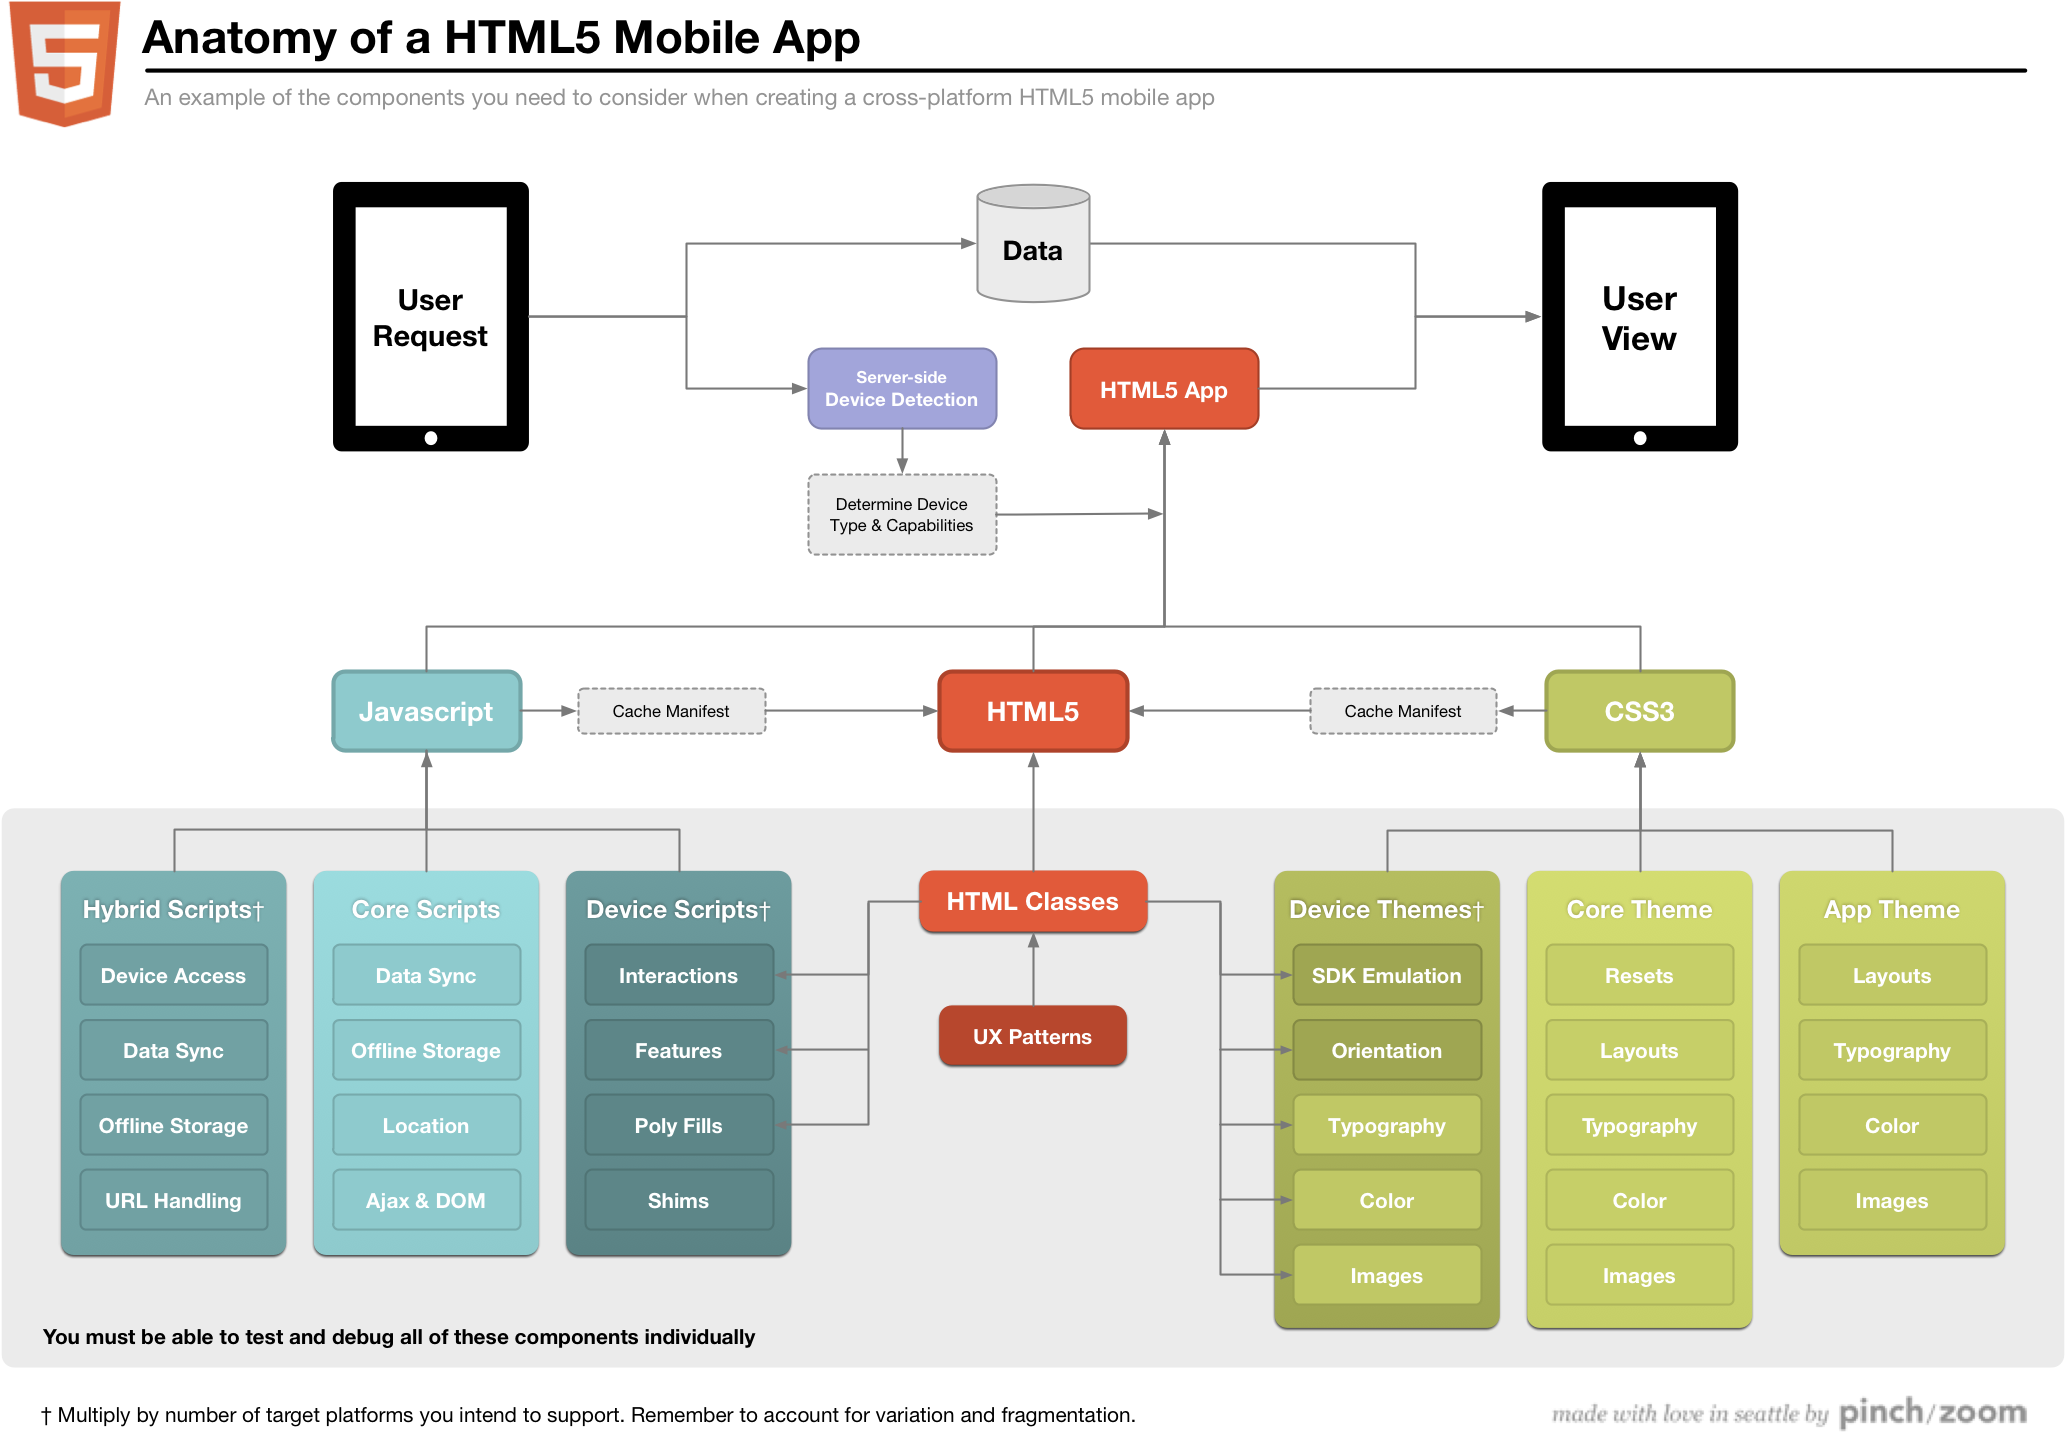
\includegraphics[width=\textwidth]{images/anatomy-of-a-html5-mobile-app.png}
  \caption{HTML5 Mobile Application Anatomy \citationneeded}
  \label{figure:anatomy-of-a-html5-mobile-app.png}
\end{figure}

\subsection{Single-Page applications}
\subsubsection{JavaScript MVC Libraries}

\subsection{Responsive Design}
\subsection{Progressive Enhancement}
\label{subsection:progressive-enhancement}

\subsection{UI Libraries}
\subsubsection{jQuery Mobile}
\subsubsection{jQTouch}
\subsubsection{Sencha Touch}

\subsection{Hybrid Applications}
\subsection{Wrapping Web Applications Application Stores}

\clearpage
\section{Performance Guidelines}
\label{section:performance-guidelines}

There are several web application performance best practices and
related guidelines. According to Souders \cite{souders2007high}, only
10--20\% of the end user response time is spent generating and
transferring the HTML document from the web server to the
client. Therefore, most of the optimization should be done in the
frontend for best improvement opportunities. Below we list the
performance guidelines defined by Souders \cite{souders2007high,
  souders2009even}.

\begin{itemize}

  % High Performance Web Sites

\item \textbf{Make Fewer HTTP Requests}

  According to Souders, 80--90\% of the end user response time is
  spent downloading components in a page other than the requested HTML
  page. Therefore, the simplest way to improve the response time is to
  reduce the number of HTTP requests needed to get all the required
  components.

  There are several ways to reducing the number of needed HTTP
  requests. Combining images into sprites, inlining images, or
  combining separate JavaScript and CSS files result in fewer
  components needed to download in a page.

\item \textbf{Use a Content Delivery Network}

  As web applications are deployed and become accessible worldwide,
  latency might become an issue for users far from the application's
  web servers. Geographically distributed servers allow for serving
  the application as close to the user as possible.

\item \textbf{Add an Expires Header}

  Avoiding a HTTP request altogether is the best option for reducing
  the response time when downloading the components in a page. Good
  caching strategies help browsers to know which resources are valid
  and for how long until they should be updated.

  The Expires header in HTTP tell the client how long a resource is
  valid, and especially far future Expires headers reduce the need for
  downloading an updating the components in a page after the initial
  download.

\item \textbf{Gzip Components}

  Compressing HTTP responses is an easy and effective way to reduce
  the size of the data needed to transfer across the
  network. Compression is supported widely in web browsers and the
  impact of reduced response sizes is huge. Using Gzip, the response
  size is reduced generally about 70\%.

\item \textbf{Put Stylesheets at the Top}

  Putting the CSS files to the top of the document allows the page to
  load progressively and the browser show visual feedback to the user
  as early as possible.

\item \textbf{Put Scripts at the Bottom}

  Because scripts block parallel downloads, they should be included to
  the page after all other resources. They also block progressive
  rendering of all content below them in the HTML document, and should
  therefore be at the bottom of the document.

\item \textbf{Avoid CSS Expressions}

  CSS expressions are a way to dynamically set CSS properties in
  Internet Explorer by evaluating a JavaScript code in a
  stylesheet. However, despite the obvious upsides, the expressions
  are evaluated at such a high frequency that they negatively impact
  the performance.

\item \textbf{Make JavaScript and CSS External}

  There are performance tradeoffs between making JavaScript and CSS
  external versus inlining them in the HTML document. In the typical
  case, however, making them external enables the browser to leverage
  the HTTP caching semantics and thus reduces the needed network
  transfer.

\item \textbf{Reduce DNS Lookups}

  Apart from cached DNS lookups, the browser typically needs 20--120
  milliseconds to look up the \abbr{IP} address for a given
  hostname. The cache lifetime of a lookup depends on the \abbr{TTL}
  value of the DNS record and having the components of a page
  distributed across several domains might accumulate into a
  noticeable response time.

  There is also a trade off between unique hostnames and allowed
  parallel connections and therefore these settings should be
  configured based on the application architecture and needs.

\item \textbf{Minify JavaScript}

  Because JavaScript is an interpreted language that must be sent to
  the web browser as source code, minifying the code reduces the
  required network transfer. Minifiers and obfuscators optimize the
  size of the source code by stripping extra whitespace and comments
  as well as renaming variable and function names to shorter ones
  without changing the interpreted behavior of the code.

\item \textbf{Avoid Redirects}

  Rerouting any component in a page takes time, and avoiding any kind
  of redirects improves the response times.

\item \textbf{Remove Duplicate Scripts}

  Including a resource several times serves no purpose but is actually
  quite common. Developers should make sure to include resources only
  once.

\item \textbf{Configure ETags}

  \abbr{ETags} are a mechanism in HTTP for servers and browsers to
  validate cached resources. The typical default values set by
  commonly used web servers might hurt performance, and should thus be
  configured properly to address the application architecture and
  needs.

\item \textbf{Make Ajax Cacheable}

  Highly dynamic web sites have a lot of \abbr{Ajax}
  \cite{garrett2005ajax} functionality, and developers should make
  sure all the requested URLs for data fetching follow the performance
  best practices such as having the proper caching in place.

  % Even Faster Web Sites

\item \textbf{Splitting the Initial Payload}

  Nowadays, web sites include a lot of resources and JavaScript
  functionality, but only a small part of the downloaded components
  are used in the typical use cases of the application. Splitting the
  resources into bundles that can be lazily downloaded when first
  needed reduces the initial payload needed to transfer on application
  startup.

\item \textbf{Loading Scripts Without Blocking}

  Most browsers block the downloads of other resources when scripts
  are being downloaded and executed. There are several ways to
  circumvent this behavior to allow browsers download scripts in
  parallel with other resources as well as with other script files.

\item \textbf{Coupling Asynchronous Scripts}

  Related to the previous item, when using parallel downloads with
  scripts that are dependent on each other, race conditions might
  occur due to the varying order of download and execution. Therefore,
  asynchronous scripts dependent on each other should be coupled to
  preserve the correct order of execution.

\item \textbf{Positioning Inline Scripts}

  Inline scripts do not introduce a HTTP request, but they can still
  block parallel downloads of other resources and they might affect
  also the progressive rendering of the page. With the correct
  positioning of the scripts, these problems can be handled properly.

\item \textbf{Writing Efficient JavaScript}

  After networking, the obvious place to optimize the runtime speed of
  a web application is the JavaScript code.

  Because the whole \abbr{UI} and the JavaScript code run in the same
  browser thread, there can be only one thing happening at a
  time. Long running functions block the UI from updating and can
  result in bad \abbr{UX}.

  Splitting the running code into properly sized chunks, appropriately
  leveraging the asynchronous patterns of JavaScript in the
  application architecture, understanding the details and slow parts
  of the DOM API, and using several JavaScript programming best
  practices can result in big improvements in the perceived
  application performance. \cite{zakas2010high}

\item \textbf{Scaling with Comet}

  For real-time data-driven applications, there are various
  optimization techniques related to optimizing the constant data
  transfer between the server and the client. The collection of there
  various technologies is unofficially called Comet.

\item \textbf{Going Beyond Gzipping}

  Although Gzipping is widely supported in web browsers, there are
  cases when it is not supported or when the support is not
  indicated. Stripping extra content such as unneeded whitespace and
  comments reduces the payload size for uncompressed responses. There
  are also ways to detect Gzip support if the client does not directly
  indicate that.

\item \textbf{Optimizing Images}

  Images typically tend to account for a large portion of the page
  weight, and since the page weight is highly correlated to the
  response time, images are a natural target for optimization. There
  are several ways to optimize images either with lossy or lossless
  conversions.

\item \textbf{Sharding Dominant Domains}

  By tuning the amount of unique hostnames used for serving all the
  resources of an application, parallel downloads can be better
  leveraged. Also, by using HTTP 1.0 with proper Keep-Alive headers or
  HTTP 1.1 with proper persistent connections the parallel downloads
  can be tuned for better performance.

\item \textbf{Flushing the Document Early}

  Some web application frameworks allow flushing parts of the document
  to the user before the whole document is generated. This enables
  progressive rendering and gives faster feedback to the user and thus
  improves the perceived performance.

\item \textbf{Using Iframes Sparingly}

  Iframes enable developers to embed a separate HTML document inside
  another document. They are useful in sandboxing external documents
  in the same view, but the iframe element is the most expensive DOM
  element related to the page performance.

\item \textbf{Simplifying CSS Selectors}

  There are several ways to choose elements in CSS stylesheets to
  apply the defined properties to. Some selectors are faster than
  others and some have terrible performance.

\end{itemize}
